\chapter{Introdução}
\setcounter{page}{11}
A história de homens e animais domésticos é uma parceria antiga que acompanhou o desenvolvimento da civilização humana, proporcionando inúmeros benefícios. Mas aquilo que antes era apenas um vínculo de apoio ou segurança sofre grandes mudanças atualmente, principalmente devido ao controle de natalidade e ao processo de urbanização, fazendo com que os animais domésticos passem a assumir um papel diferenciado nas relações intrafamiliares, de modo que o proprietário chega a identificá-los como membros da família e proporcionam privilégios que antes eram partilhados apenas por seres humanos.
\\
\indent
De acordo com o crescimento populacional, muitos animais são adotados por um motivo sentimental, pois algumas pessoas acabam priorizando a atividade profissional, deixando para outro momento a formação de uma família.
\\
\indent
Os animais domésticos preenchem esse espaço, tornando assim uma transferência social mútua, na qual um complementa a vida um do outro, ou seja, há um beneficio para ambas as partes, como no mutualismo. Segundo os dados do Censo 2013 divulgados pelo IBGE (Instituto Brasileiro de Geografia e Estatística), aproximadamente 44,3\% (equivalente a 52,2 milhões) dos domicílios do país possuem pelo menos um cão e 17,7\% (equivalente a 11,5 milhões) possuem pelo menos um gato, fora outros animais criados nos lares brasileiros, que fazem com que esses números aumentem à cerca de 100 milhões. Isso confirma que há no Brasil mais animais domésticos do que crianças (45 milhões) até os onze anos (ARIAS, 2015). 
\\
\indent
Segundo o estudo liderado por Allen McConnel, da Universidade de Miami, publicado no site do Journal of Personality and Social Psychology, pessoas que convivem com animais de estimação "têm mais qualidade de vida e conseguem resolver melhor diferenças individuais que as que não têm animal de estimação" (VEJA, 2015). O estudo também afirma que a criação de animais estimula o bom humor, a autoestima, a diversão,  afasta o sedentarismo e depressão, atuando ainda nos sentimentos de solidariedade, respeito, cumplicidade e amizade sejam adultas ou crianças melhorando em muito dos casos a qualidade de vida dos seus proprietários. Além disso, são demonstradas que grande parte das pessoas que convivem com animais vão menos ao médico e a recuperação de determinadas doenças tornam-se mais rápidas. 
\\
\indent
Mesmo com tantos benefícios, ainda há donos que não tratam seus animais com o devido cuidado, principalmente com relação a vacinas e medicamentos. Segundo os dados do censo do IBGE, cerca 75,4\% dos lares entrevistados nunca vacinaram seus animais ou deram a vacina num período de um ano antes da data de pesquisa. E isso ocorre muitas vezes por falta de informações necessárias que situem os donos, simplesmente por não haver uma integração comum, rápida e eficiente entre a comunidade de donos de animais de estimação, veterinários, clínicas e vendedores de produtos ou serviços, em conjunto com as mais variadas redes sociais.

\section{Problemática}

Um dos grandes problemas para quem tem animais de estimação é quando estes fogem, pois normalmente não possuem nenhuma identificação, causando uma experiência angustiante ao proprietário, a família e principalmente ao {\it pet} (animal), devido aos riscos que correm. Tornando ainda mais difícil quando se tem crianças em casa. Aflitos, muitos proprietários não sabem quais medidas tomar e pensam, instantaneamente, em compartilhar fotos e dados do seu animal em redes sociais, sites de procura, entre outros. Mas, nem sempre há êxito em tais medidas.
\\
\indent
Outro dado importante, segundo a Associação pelos animais, é que desde 2005, a maioria desses {\it pets} perdidos são encontrados e recolhidos por pessoas comuns (Diferentes de veterinários, clínicas ou canis), como mostrado na Figura 1.


\begin{figure}[!htb]
	\centering
	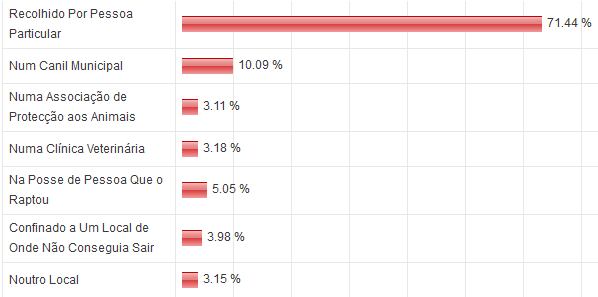
\includegraphics[scale=0.70
	]{imagens/animais}
	\caption{Gráfico com os principais destinos de animais domésticos perdidos}
	Fonte: encontra-me.org – Associação pelos animais. 2005 – 2015.
	\label{Rotulo}
\end{figure}
\newpage
Na maioria dos casos, as pessoas que encontram esses {\it pets} não imaginam que estes possuem proprietários, principalmente pelo animal não possuir nenhum mecanismo que os identifique. Assim essas pessoas acabam recolhendo os animais das ruas, para seus lares. 
\\
\indent
Além disso, o fato do animal não ter um sistema eficaz de identificação, dificulta bastante o seu tratamento, já que não é possível obter de forma eficaz aos seus históricos hospitalares, medicamentos, veterinários particulares e as clínicas mais confiáveis. Dificultando ainda o reconhecimento de doenças que o mesmo tem, impedindo assim, um tratamento ou a execução de uma cirurgia, caso este seja encontrado num difícil estado de saúde.  

\section{Objetivos}
Na seguinte seção serão abordados os objetivos do projeto, dividos em: gerais e específicos.
\subsection{Objetivos Gerais}
Procurou-se desenvolver uma rede social diferenciada, capaz de integrar os animais de estimação ao meio social digital, além disso, buscou-se Proporcionar o aprendizado e a vivência de uma equipe de desenvolvimento com troca de experiências e conhecimento.

\subsection{Objetivos Específicos}
\textbf{•} Facilitar na identificação dos proprietários dos animais perdidos, para que esse seja comunicado acerca do seu pet, através do QR Code;
\\
\indent
\textbf{•} Proporcionar uma integração via rede social, que forneça uma maior praticidade numa consulta veterinária;
\\
\indent
\textbf{•} Exibir dados clínicos para que o veterinário fique ciente das medicações do animal e de doenças que ele teve em outras ocasiões;
\\
\indent
\textbf{•} Promover clínicas, veterinários, pet shops favoritos;
\\
\indent
\textbf{•} Permitir ao dono dos animais, compartilhar as tarefas diárias do seu animal, nas mais variadas redes sociais.

\section{Justificativas}

Como dito, observa-se que o mercado de animais de estimação é crescente, tornando-se assim, necessária a promoção de ideias para esses novos serviços. Isso ocorre porque a cada dia é considerável o aumento de benefícios que animais proporcionam aos humanos. Tornando assim, mais comum as famílias adotarem um {\it pet}, e tratá-los como verdadeiros membros da família.
\\
\indent
Mesmo querendo o melhor para os seus animais, 
%Sabe-se que os donos dos animais sempre procuram o melhor para os seus animais, 
muitos donos acabam não conseguindo prover-lhes melhores condições, seja com problemas financeiros, grandes distâncias de clínicias, entre outros fatores. Nota-se também, que a sociedade atual está sempre rodeada por tecnologia, seja utilizando redes sociais, aplicativos móveis dentre outros.
\\
\indent
Portanto, identificando a importância desses pontos para a sociedade atual, o ePuppy surge como uma rede social buscando, conciliar as mais variadas comunidades (clínicas, veterinários e vendedores de produtos e serviços) com os proprietários que buscam sempre o melhor para os seus {\it pets}, seja no aprofundamento de informações, consultas e serviços diferenciados (gerenciador de e-mails e compartilhamento de conhecimento), facilitando também o encontro destes, por meio de coleiras personalizadas com {\it QR Code}.


\section{Organização do Documento}

O presente trabalho está moldado em seis capítulos. Através desde capítulo, foi apresentada a introdução do trabalho, relacionando justificativa, problemática, objetivos e metodologia utilizada. No segundo capítulo (Fundamentação Teórica), será apresentado o embasamento do trabalho de acordo com alguns estudiosos da área. Ao longo do capítulo 3 (Redes sociais e o ePuppy), será abordado uma breve pesquisa sobre redes sociais, e suas principais características, relacionando com o ePuppy e sistemas relacionados. O capítulo 4 (Análise dos requisitos), discorrerá sobre as principais formas de elicitação de requisitos utilizadas, casos de uso e diagramas e entidade-relacionamento. O capitulo 5 (Análise dos resultados), descreverá todas as funcionalidades implementadas no sistema. E o capítulo 6 (Considerações Finais), apresentará as conclusões embasadas nas pesquisas realizadas e sugestões para trabalhos futuros.



\nocite{Nascimento2014}
\nocite{Aguilar2015}
\nocite{Anaya2015}
\nocite{Arias2015}
\nocite{G12015}
\nocite{Gazzana2015}
\nocite{Veja2015}
